\section{第5問：3次元HPモデルと学習形質の遺伝}
\label{sec:hp}

\subsection{問題設定と比較の考え方}
HPモデルはアミノ酸を疎水性Hと極性Pの2種類に簡略化し、鎖を格子上に置くモデルである。本実験では立方格子を用い、同じ格子点に2残基を置かず、鎖の隣接残基間のマンハッタン距離を1とする。鎖に沿って隣り合わないH同士が格子上で接したときにエネルギーを1下げる。
\begin{equation}
 E(r)=-C_{HH}(r).
\end{equation}
ここで$C_{HH}$は、$j>i+1$、$s_i=s_j=H$、$\|r_i-r_j\|_1=1$をすべて満たす残基対$(i,j)$の数である。したがって小さい$E$ほどよい。P間接触とH--P接触には得点を与えない。

集団内の構造を交叉と突然変異で改善する考え方はUngerとMoultの先行研究を参考にした\footnote{R. Unger and J. Moult, ``Genetic Algorithms for Protein Folding Simulations,'' \emph{J. Mol. Biol.}, 231(1), 75--81, 1993. \url{https://doi.org/10.1006/jmbi.1993.1258}}。実装は独自に作成し、同一の実行可能解空間と遺伝演算に対して、学習結果を評価と遺伝のどちらに使うかだけを変更した。実タンパク質の立体構造や折り畳み時間を予測するモデルではなく、探索と学習の相互作用を調べる計算実験である。

\subsection{遺伝子型・表現型と実行可能性}
遺伝子型は原点を始点とする3次元整数座標列である。これは6方向の結合ベクトル列と相互変換できる。重なった構造を罰点で扱う方式では、重なりの解消とH核の形成という異なる課題が適合度に混ざる。そのため、初期化・交叉・突然変異のすべてで自己回避歩行を保持した。

初期集団は空いている隣接格子点から逐次ランダムに成長させ、成長が行き詰まった場合だけ作り直した。交叉は親Aの前半と親Bの後半を、接続点を共有するよう平行移動・回転してつなぐ。回転は立方体の24通りの正規回転から選ぶ。最大8回試して重なりのない子を得られなければ親Aを返す。突然変異は、鎖の後半を回転するpivot変異を確率0.65、末端側の最大12残基を再成長する変異を確率0.35で選ぶ。pivotは最大12回、再成長は最大6回試し、成功しなければ元の構造を残す。失敗も実行時間には含まれる。

学習操作$L(x)$は、末端残基の移動、正方形の対角側へのcorner flip、連続2残基のcrankshaft移動をすべて調べ、エネルギーの減少が最大の移動を採用する最急降下法である。改善がなくなるまで繰り返し、反復回数の打切りは設けない。整数エネルギーが厳密に減少し、下限を持つので必ず終了する。ここで得る局所最適性は、この明示した小近傍に関するものである。等エネルギーの平坦部の横断や大きなpivot操作は含まない。

1回の近傍移動で変わる残基は1個か2個なので、接触エネルギーは変更残基に接する対だけから差分計算した。全再計算との一致、結合長、自己回避性、局所探索終了時の全近傍に対する非改善性を自動テストで確認した。

\subsection{3種類のGAを混同しない実装}
ダーウィン型は遺伝子型$x$の$E(x)$を評価し、そのまま子の生成に使う。ボールドウィン型は$E(L(x))$を評価に使うが、交叉・変異の入力は学習前の$x$である。ラマルク型は$L(x)$自体を遺伝子型に書き戻す。これらを表\ref{tab:hp-inheritance}に示す。選択はエネルギーの小さい個体を優遇する。

\begin{table}[htbp]
\centering
\small
\caption{適合度と継承対象を分けた実装。}
\label{tab:hp-inheritance}
\begin{tabular}{lll}
\hline
型 & 評価する値 & 子に使う構造\\
\hline
Darwin & $E(x)$ & $x$\\
Baldwin & $E(L(x))$ & $x$\\
Lamarck & $E(L(x))$ & $L(x)$\\
\hline
\end{tabular}
\end{table}

特に、ボールドウィン型でエリートとして保存する遺伝子型も$x$のままにした。改善後の構造だけを保存すると、意図せずラマルク型になってしまう。集団の学習前エネルギーと学習後適合度を別々に記録し、両者の違いを検査可能にした。一方、報告用の最良解アーカイブには、局所探索中を含め、実際に評価したすべての構造を記録した。このアーカイブは親選択や集団への再投入には用いない。

\subsection{配列の検査と実験条件}
課題ページの圧縮表記を展開するパーサを作り、掲載された10配列を機械的に検査した。その結果、\textbf{「配列48」とされた第1・第10配列は、掲載文字列をそのまま展開すると47残基だった}。第2--第9配列は48残基である。欠落文字を推測して補うと問題を変更するため、原文と警告を保存し、48残基の比較には第2・第3・第4配列を用いた。課題ページに記載された参照エネルギーは、それぞれ$-34,-34,-33$である。以下ではこれらをs48\_02、s48\_03、s48\_04と呼ぶ。

簡単な対照例として、独自配列toy10=$H^2P^2H^2P^2H^2$、toy20=$(H^2P^2)^4H^4$を加えた。toy10は最初の結合を$+x$方向に固定して、自己回避歩行を全列挙した。この固定は剛体回転による対称性の除去であり、最適値を変えない。完全な歩行308,981本、途中の歩行を含む390,769ノードを調べ、\textbf{最適値$E=-4$を厳密に確認した}。toy20と48残基配列には全列挙による最適性の保証はない。

各配列・各手法についてseed 0--4の5試行を行い、計75試行とした。各seedの初期集団は3手法で同一にし、初期化とその後の遺伝操作には別の乱数系列を使った。集団サイズ32、トーナメントサイズ3、エリート2、交叉確率0.8、変異確率0.9、ランダム移入確率0.03は共通である。エリートは再評価しない。

比較の基準は、(a)局所探索の候補評価も含めた30,000構造の評価、(b)60世代、(c)実測時間、の3通りとした。評価回数が30,000に達した瞬間に、実際にその時点までに観測した最良解を保存する。局所探索の途中で閾値に達した場合でも、後から得た改善解は(a)に含めない。その後の局所探索は完了させ、別の条件である(b)を取得するまで走らせる。反対にダーウィン型は60世代での結果を保存後、30,000評価まで続ける。この設計により、評価予算の超過と局所最適性の取り違えを防いだ。

実行環境はmacOS 15.5、arm64、Python 3.9.6であり、75試行全体で9,939,381回の構造評価を行った。各試行を逐次実行し、共通の初期構造生成を前処理として除外し、初期集団の評価から計時した。その後の選択、遺伝操作、局所探索と記録処理を時間に含む。同じホストでは他課題の処理が動く場合があるため、時間はこの実装と環境での観測値として解釈する。

\subsection{解の品質と探索効率}
表\ref{tab:hp-main}は5試行の平均を示す。toy10は全手法・全seedで厳密最適値$-4$に到達した。一方、48残基配列では、どの資源を揃えるかによって順位が変化した。

\begin{table}[htbp]
\centering
\caption{最良エネルギーの平均。同評価数は30,000構造、同世代数は60世代、秒は60世代までの平均経過時間。小さいエネルギーがよい。}
\label{tab:hp-main}
\small
\begin{tabular}{llrrr}
\hline
配列 & 手法 & 同評価数 & 同世代数 & 秒\\
\hline
toy10 & Darwin & -4.0 & -4.0 & 0.06\\
toy10 & Baldwin & -4.0 & -4.0 & 0.29\\
toy10 & Lamarck & -4.0 & -4.0 & 0.24\\
toy20 & Darwin & -11.4 & -11.0 & 0.12\\
toy20 & Baldwin & -11.0 & -11.8 & 0.78\\
toy20 & Lamarck & -11.8 & -12.2 & 0.47\\
s48\_02 & Darwin & -25.2 & -19.4 & 0.24\\
s48\_02 & Baldwin & -16.0 & -23.2 & 2.63\\
s48\_02 & Lamarck & -19.2 & -22.8 & 0.97\\
s48\_03 & Darwin & -22.6 & -20.2 & 0.25\\
s48\_03 & Baldwin & -15.8 & -21.8 & 2.20\\
s48\_03 & Lamarck & -20.8 & -24.4 & 0.84\\
s48\_04 & Darwin & -19.6 & -17.4 & 0.26\\
s48\_04 & Baldwin & -15.6 & -22.8 & 2.11\\
s48\_04 & Lamarck & -19.4 & -22.2 & 0.86\\
\hline
\end{tabular}

\end{table}

\begin{figure*}[t]
\centering
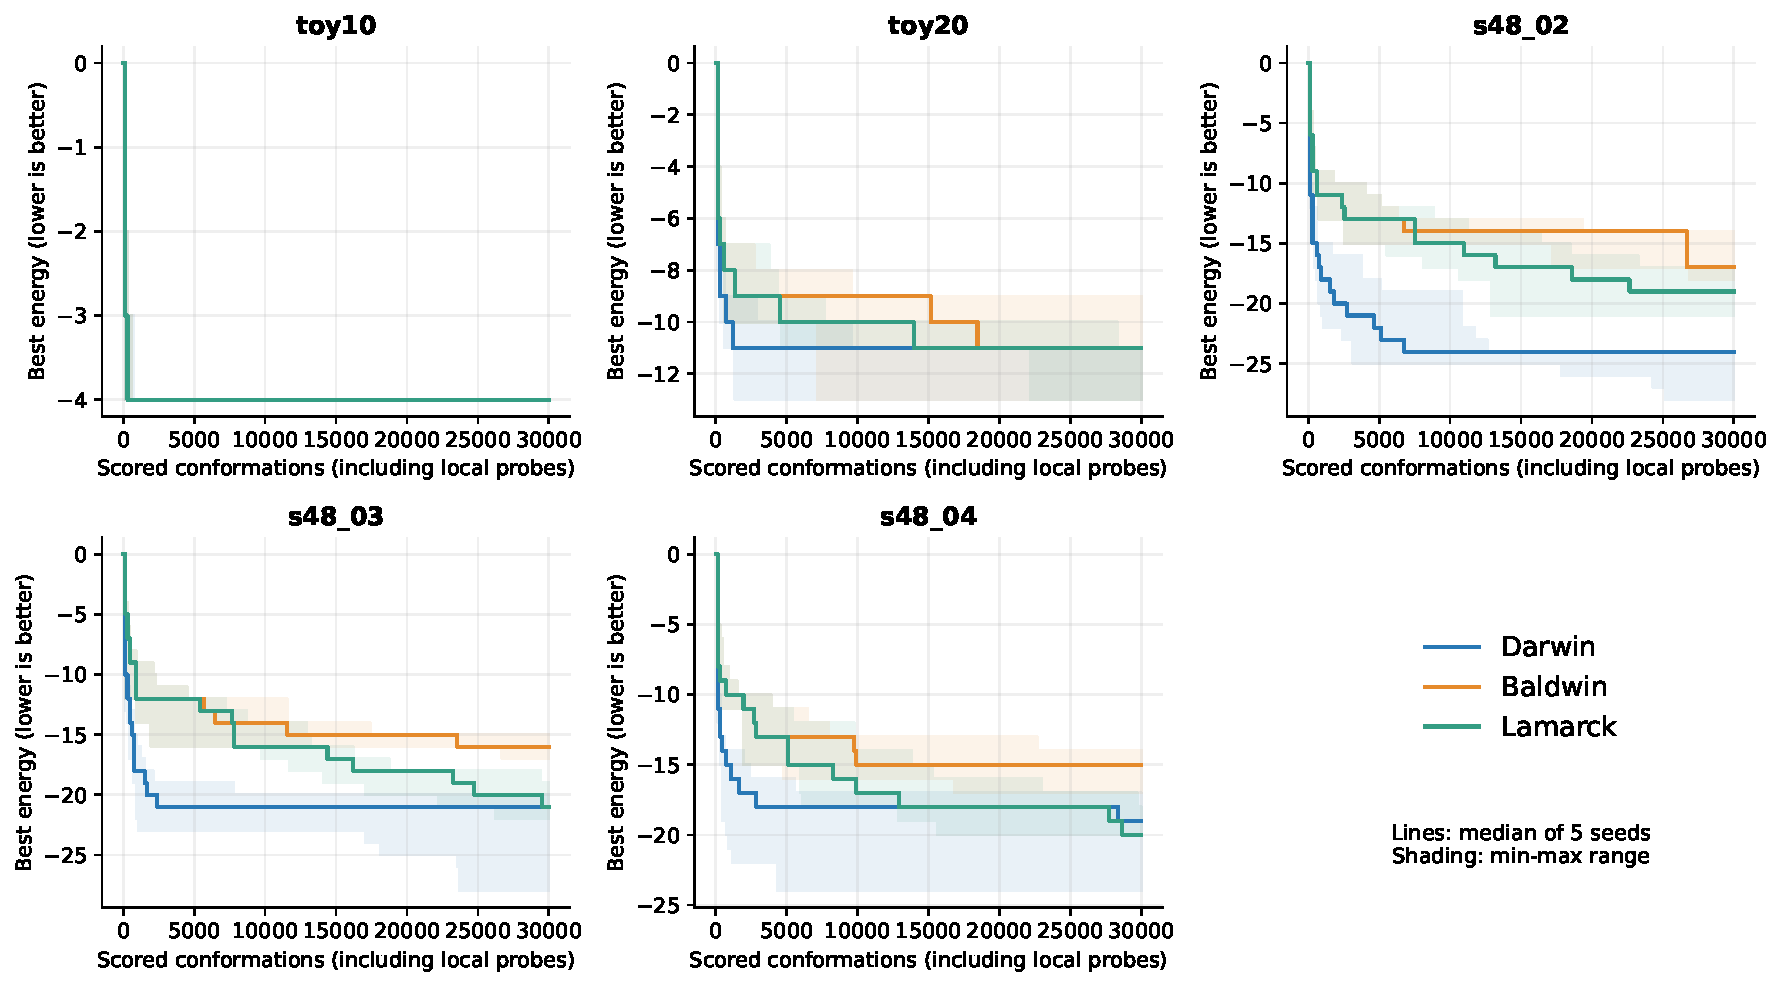
\includegraphics[width=\textwidth]{05/results/convergence_evaluations.pdf}
\caption{評価した構造数を揃えた比較。線は5試行の中央値、陰影は最小値--最大値であり信頼区間ではない。局所探索の近傍候補も1評価として数える。}
\label{fig:hp-eval}
\end{figure*}

\begin{figure*}[t]
\centering
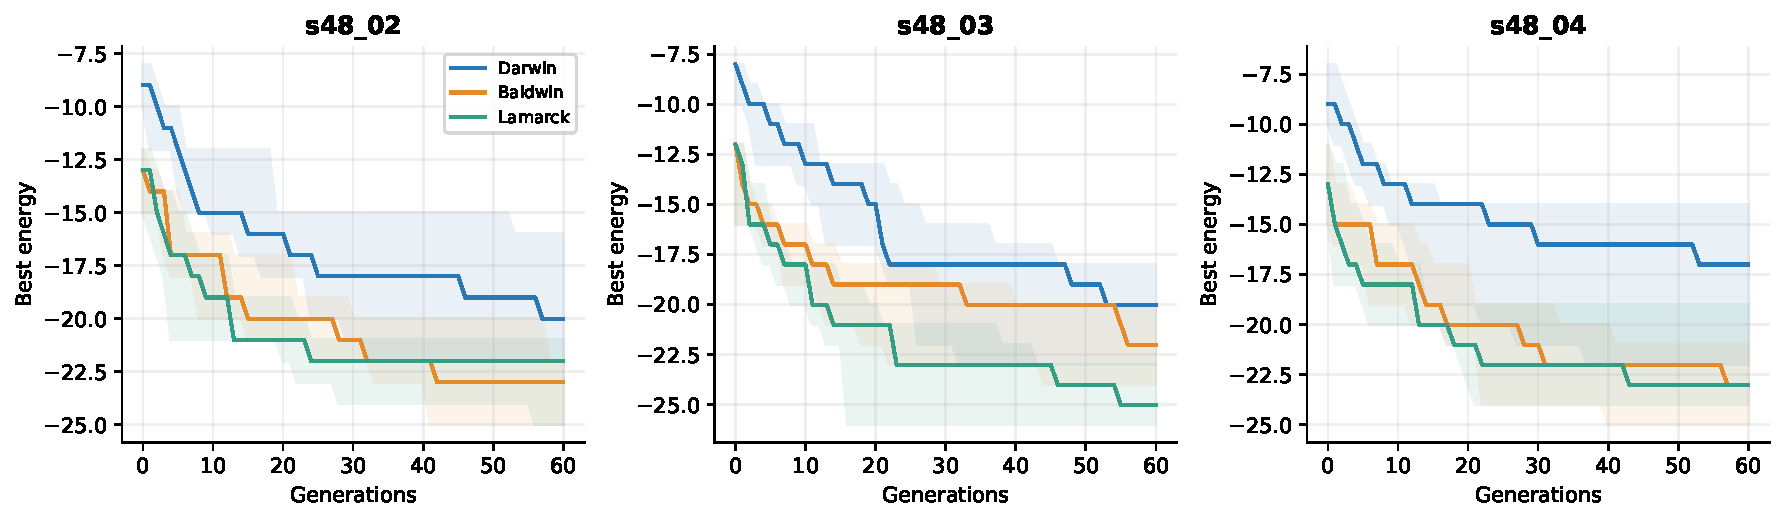
\includegraphics[width=\textwidth]{05/results/convergence_generations.pdf}
\caption{同じ60世代での比較。局所探索による1世代当たりの計算量は共通ではない。}
\label{fig:hp-generation}
\end{figure*}

30,000評価に限ると、s48\_02の平均値はDarwin $-25.2$、Baldwin $-16.0$、Lamarck $-19.2$であり、ダーウィン型が優れていた。試行範囲はそれぞれ$[-28,-24]$、$[-18,-14]$、$[-21,-17]$である。s48\_03でも$-22.6,-15.8,-20.8$と同じ順序であり、s48\_04ではDarwin $-19.6$とLamarck $-19.4$が近かった。局所探索には多くの候補評価が必要なので、少ない評価数を世代更新と大きな構造変化に使う方法が有利になったと解釈できる。

60世代に揃えると、s48\_02は$-19.4,-23.2,-22.8$、s48\_03は$-20.2,-21.8,-24.4$、s48\_04は$-17.4,-22.8,-22.2$となり、学習を行う2手法がいずれもダーウィン型を上回った。例えばs48\_02の60世代までの平均評価数は、Darwin 1,832、Baldwin 449,423、Lamarck 121,913である。ボールドウィン型は改善後の構造を遺伝しないため、各子について再び学習する費用が大きい。したがって、同世代数の優位だけから計算効率の優位を結論することはできない。

\begin{figure*}[t]
\centering
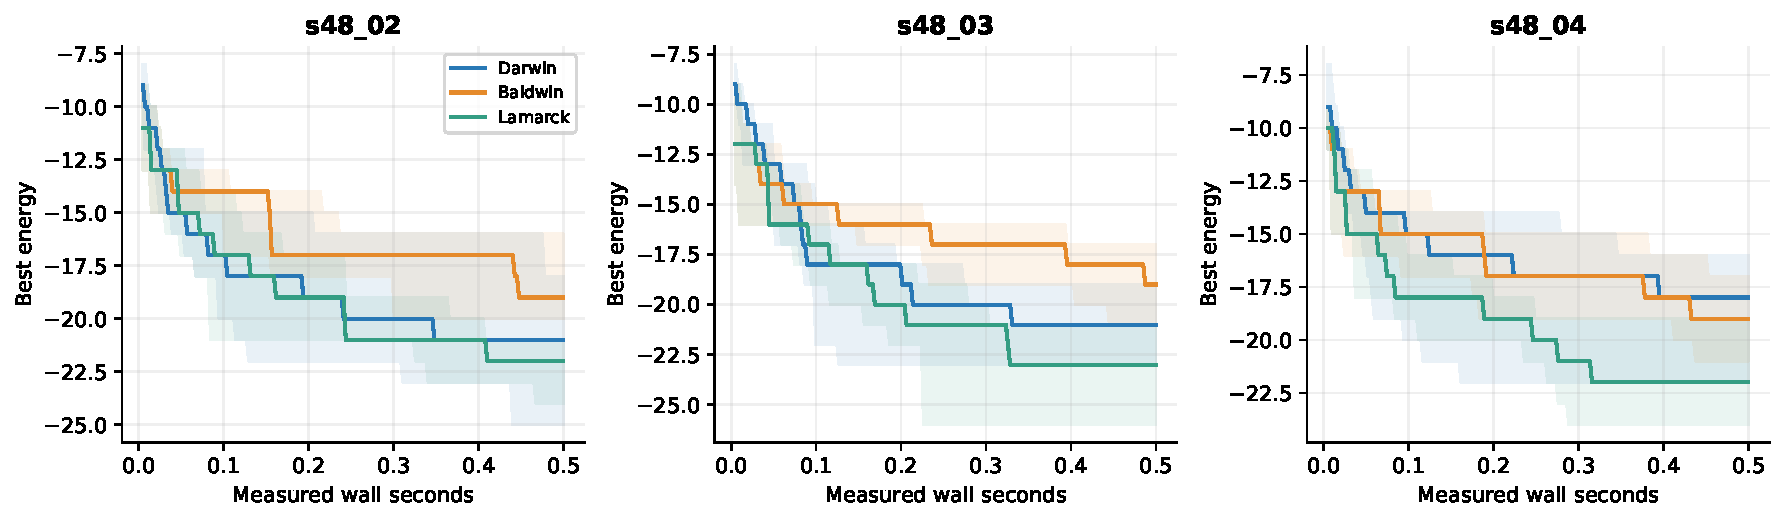
\includegraphics[width=\textwidth]{05/results/convergence_time.pdf}
\caption{48残基の各試行に共通の実測0.5秒までの比較。線は中央値、陰影は試行範囲。局所近傍の差分評価と遺伝操作の費用差が、評価回数基準の順位に影響する。}
\label{fig:hp-time}
\end{figure*}

実時間も揃えると、0.5秒時点の平均値はs48\_02で$-21.6,-18.4,-22.4$、s48\_03で$-20.8,-18.8,-23.2$、s48\_04で$-18.6,-18.8,-22.0$であり、この測定ではラマルク型が3配列とも最もよかった。30,000評価までの平均時間は、例えばs48\_02で4.29秒、0.17秒、0.22秒と大きく異なる。局所探索は変更残基だけを差分評価できる一方、ダーウィン型は1評価ごとに交叉・変異・全接触計算を行うためである。\textbf{「1評価」を同じCPU費用と見なすと、結論を誤る}ことが本実験の主要な知見である。0.5秒比較は保存した改善イベントの時刻から集計したもので、異なる機械でも同じ優劣を保証するものではない。

\subsection{目標水準へ到達するまでの世代と時間}
最良値の比較を補うため、保存済みログに対する補助解析として、s48\_02に共通目標$E\leq-20$を設定した。
これは最適値ではなく、実験後に定めた到達水準である。
60世代以内での初到達を調べ、未達試行は打切りとして残した。
秒は改善イベントの時刻、世代は到達を確認できた最初の世代末の記録を用いる。
\begin{table}[tb]\centering\small
\caption{s48\_02で$E\leq-20$への到達。世代と秒は成功試行のみの中央値であり、全試行の平均ではない。}
\begin{tabular}{lrrr}\hline
手法 & 到達数 & 世代 & 秒\\\hline
Darwin & 3/5 & 51 & 0.205\\
Baldwin & 5/5 & 15 & 0.591\\
Lamarck & 5/5 & 13 & 0.243\\
\hline\end{tabular}

\end{table}
Darwinの成功は3/5、BaldwinとLamarckは5/5であった。
成功した試行ではDarwinの秒の中央値が小さい一方、BaldwinとLamarckは少ない世代でより確実にこの水準へ到達した。
成功試行だけの時間を見れば未達2試行を無視することになるため、到達率との併記が必要である。
目標値や観測期間を変えれば順位も変わりうる。
解析コード\texttt{time\_to\_threshold.py}と各試行の打切り状態も保存した。

\subsection{学習効果と集団の多様性}
学習前の遺伝子型と学習後の表現型を分けて観察すると、手法の違いが明瞭になる。s48\_02、seed 0、60世代のボールドウィン型では、集団の平均遺伝子型エネルギーが$-5.16$、平均学習後適合度が$-14.97$であり、平均9.81接触分の学習改善が残っていた。集団内の最良遺伝子型は$-9$、最良学習後構造は$-23$だった。評価結果が良好でも、その構造自体を継承しているわけではないことが数値から確認できる。

\begin{figure*}[t]
\centering
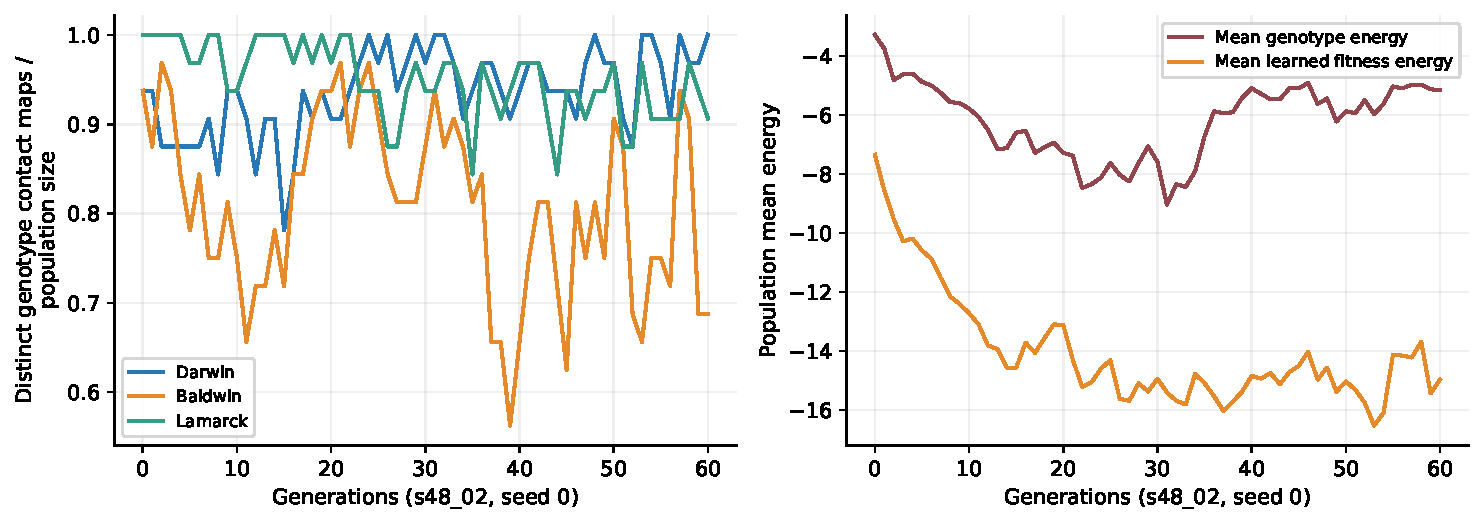
\includegraphics[width=\textwidth]{05/results/learning_and_diversity.pdf}
\caption{s48\_02、seed 0の診断。左は集団内で異なる遺伝子型接触マップの比率、右はBaldwinの学習前後の平均エネルギー。接触マップは回転・平行移動に不変だが、同じ接触集合の異なる構造を区別しない。}
\label{fig:hp-diagnostic}
\end{figure*}

多様性は、集団中の異なるH--H接触集合の個数を集団サイズで割って測った。s48\_02、60世代での5試行平均はDarwin 0.931、Baldwin 0.769、Lamarck 0.925であり、ラマルク型が常に最も多様性を失う、という単純な予想は支持されなかった。接触集合は構造の完全な識別子ではないが、座標の剛体回転だけで見かけ上の多様性が増える問題を避けられる。ここでは移入と大きな変異を併用しており、これらの設定によっても収束の仕方は変わる。

\begin{figure*}[t]
\centering
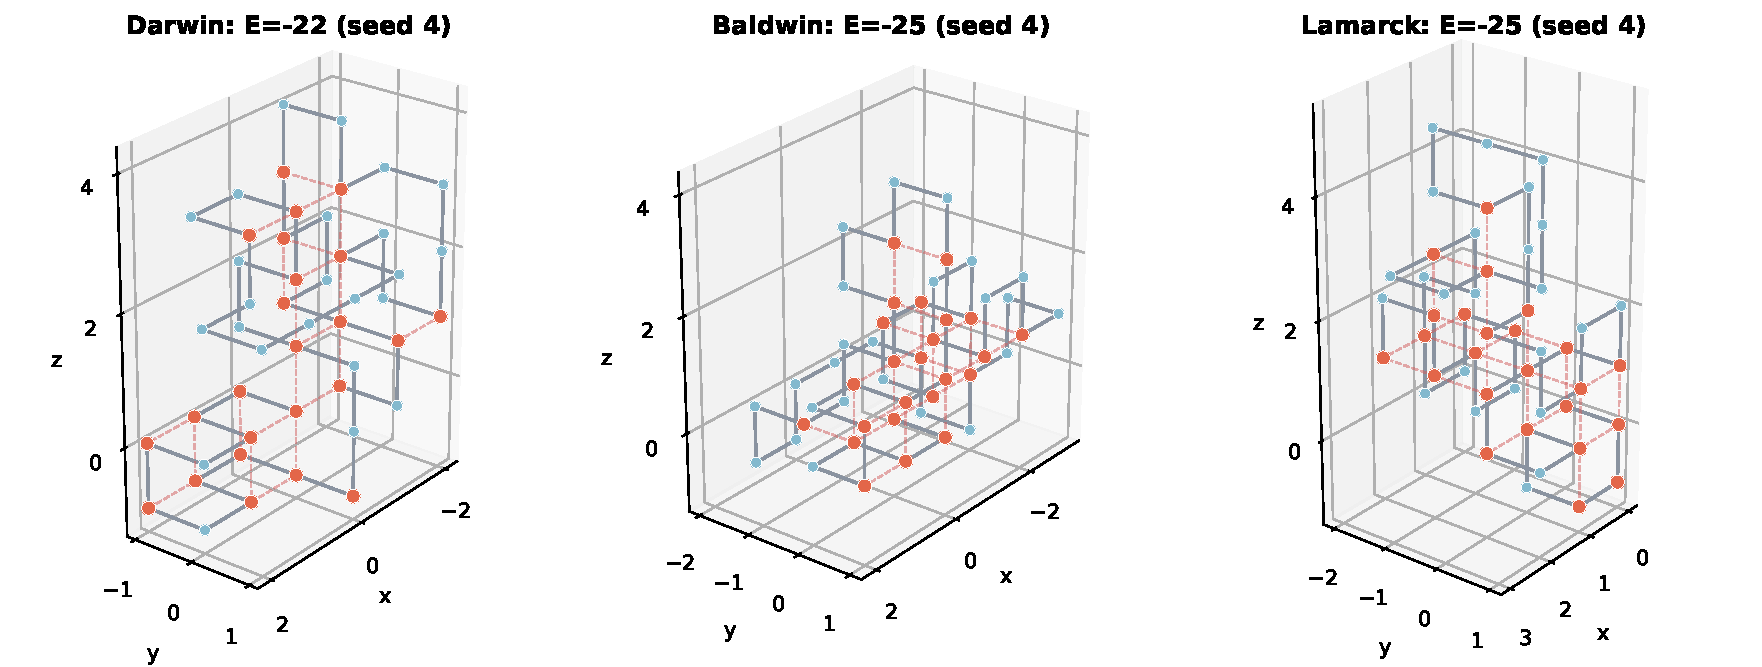
\includegraphics[width=\textwidth]{05/results/folds_3d.pdf}
\caption{s48\_02で60世代時点の最良seedの構造。橙はH、青はP、灰線は鎖、赤の破線は非共有結合H--H接触。Darwin $-22$、Baldwin $-25$、Lamarck $-25$である。異なる評価予算の最良解を混ぜていない。}
\label{fig:hp-folds}
\end{figure*}

\subsection{限界と改善案}
48残基の参照値$-34,-34,-33$は未達成であり、大域最適性は主張できない。小近傍による厳密な局所最適性は、大きな構造移動で改善できないことを意味しない。特にエネルギーが同じ平坦な地形は厳密降下だけでは横断できない。改善案として、非改善移動を一定確率で許す学習、複数の温度を持つ集団、局所学習を適用する個体の割合の適応制御が考えられる。ただし、それらを導入する場合も学習内の費用を計上し、同世代・同評価数・同時間の比較を併記すべきである。

5試行はばらつきを観察するための反復であり、普遍的な優劣や統計的有意差を示すものではない。初期集団は共通だが、学習によって選択された親が変わるため、その後の探索軌道は対応しない。今後はseed数、配列数、交叉不成立率、局所学習費用を増やして評価したい。講義については、学習を適合度だけに反映する場合と遺伝子型に書き戻す場合を、同じ構造の図と費用のグラフで並べると理解が深まると考える。

\subsection{コードと再現手順}
\texttt{hp\_model.py}に構造と遺伝演算、\texttt{experiment.py}に継承規則と計測、\texttt{analyze.py}に図表生成を分離した。\texttt{exact\_toy.py}が小規模厳密解、\texttt{test\_hp\_model.py}が構造・差分・学習規則の検査を担う。配列原文、警告、seed、全改善イベント、各世代の生データと実行環境を保存した。実行コマンドは第5問フォルダのREADMEに示す。

\repolink{05}
